\documentclass[conference]{IEEEtran}
\IEEEoverridecommandlockouts
% The preceding line is only needed to identify funding in the first footnote. If that is unneeded, please comment it out.
\usepackage{cite}
\usepackage{amsmath,amssymb,amsfonts}
\usepackage{algorithmic}
\usepackage{graphicx}
\usepackage{textcomp}
\usepackage{xcolor}
\usepackage{tikz}
\usetikzlibrary{arrows.meta, positioning, fit, backgrounds, calc}
\def\BibTeX{{\rm B\kern-.05em{\sc i\kern-.025em b}\kern-.08em
    T\kern-.1667em\lower.7ex\hbox{E}\kern-.125emX}}
\begin{document}

\title{MANTIS — Modular Agent Network Testbed for Instrumentation and Security in Multi-Agent Banking Systems

\thanks{Identify applicable funding agency here. If none, delete this.}
}

\author{\IEEEauthorblockN{1\textsuperscript{st} Given Name Surname}
\IEEEauthorblockA{\textit{dept. name of organization (of Aff.)} \\
\textit{name of organization (of Aff.)}\\
City, Country \\
email address or ORCID}
\and
\IEEEauthorblockN{2\textsuperscript{nd} Given Name Surname}
\IEEEauthorblockA{\textit{dept. name of organization (of Aff.)} \\
\textit{name of organization (of Aff.)}\\
City, Country \\
email address or ORCID}
\and
\IEEEauthorblockN{3\textsuperscript{rd} Given Name Surname}
\IEEEauthorblockA{\textit{dept. name of organization (of Aff.)} \\
\textit{name of organization (of Aff.)}\\
City, Country \\
email address or ORCID}
\and
\IEEEauthorblockN{4\textsuperscript{th} Given Name Surname}
\IEEEauthorblockA{\textit{dept. name of organization (of Aff.)} \\
\textit{name of organization (of Aff.)}\\
City, Country \\
email address or ORCID}
\and
\IEEEauthorblockN{5\textsuperscript{th} Given Name Surname}
\IEEEauthorblockA{\textit{dept. name of organization (of Aff.)} \\
\textit{name of organization (of Aff.)}\\
City, Country \\
email address or ORCID}
\and
\IEEEauthorblockN{6\textsuperscript{th} Given Name Surname}
\IEEEauthorblockA{\textit{dept. name of organization (of Aff.)} \\
\textit{name of organization (of Aff.)}\\
City, Country \\
email address or ORCID}
}

\maketitle

\begin{abstract}
Multi-agent systems built on large language models (LLMs) are increasingly deployed in banking for transaction monitoring, operations planning, and end-of-day reconciliation, yet there is no standard, reusable way to evaluate such systems under adversarial conditions without either rewriting the framework core or the business workflow logic being tested. We present MANTIS (Modular Agent Network Testbed for Instrumentation and Security), a configuration-driven testbed built around a banking multi-agent system spanning front-, mid-, and back-office workflows. MANTIS instruments five fixed control points (input, agent, interaction, tool, and output) through a hook bus that lets an experimenter declare an attack or failure condition entirely in YAML, register it as a plugin against the same interface used by every other plugin, and leave the underlying banking agents unmodified. Every run produces a signed manifest (configuration hash, seed, and environment metadata), a complete OpenTelemetry- and MLflow-integrated trace, and an automated evaluation of tool-use correctness and terminal-state outcome. We describe the architecture, the banking runtime adapter covering 31 agents and 19 tools across three domains, five concrete attack configurations spanning all three domains, and the observability and evaluation pipeline. We report live-verified evidence that all five control points behave as intended, together with a case study in why that verification has to inspect the emitted security event rather than trust a clean process exit: doing so surfaced a real, previously-undetected bug in one attack plugin's argument matching against the underlying agent framework, silently present since the plugin was written, which we diagnose against the framework's own source and fix. A tool-calling-capable mock model and a volume-scaling benchmark mode isolate instrumentation overhead from two confounds in turn -- LLM sampling latency and per-process startup cost -- arriving at a direct, repeated-trial measurement of instrumentation overhead under 1\%, together with a contention-controlled end-to-end comparison in the same direction and of comparable magnitude.
\end{abstract}

\begin{IEEEkeywords}
multi-agent systems, adversarial security, large language models, banking, observability, benchmarking, red teaming
\end{IEEEkeywords}

\section{Introduction}

Large language model (LLM) agents are moving from single-turn assistants into orchestrated multi-agent systems that carry out multi-step business processes. In banking specifically, recent work has proposed multi-agent frameworks for anomaly detection in financial markets \cite{anomaly_detection_finance} and for credit assessment \cite{masca_credit}, each decomposing a task across specialized agents -- a pattern that mirrors how a bank actually organizes front-, mid-, and back-office work today.

That same decomposition is also where new security risk enters. Safety properties established for a single chat model do not transfer to a system where behavior emerges from message passing, tool invocation, and routing decisions across multiple agents \cite{agentic_security_survey}. Recent attacks demonstrate that inter-agent communication itself is an exploitable surface: prompt injection can propagate from one agent to another like an infection \cite{prompt_infection}, and an adversary positioned between two agents can intercept and rewrite the messages passing between them without ever touching either agent's model weights or prompts \cite{aitm_communication_attacks}. A survey of agentic security threats and defenses concludes that most current defenses evaluated in isolation can be bypassed by an adaptive attacker \cite{agentic_security_survey}, underscoring that security evaluation for these systems needs to happen at the level of the deployed multi-agent system, not the underlying model.

Despite this, there is no widely available testbed that lets a researcher take a \emph{realistic, domain-specific} multi-agent system and run controlled adversarial experiments against it without either reimplementing the orchestration framework or editing the business logic under test. General-purpose red-teaming benchmarks for LLM agents exist \cite{redagentbench}, but they are typically domain-agnostic and are not designed to instrument an existing, unmodified business workflow at fixed points chosen for their security relevance.

This paper presents MANTIS, a modular, configuration-driven testbed built directly on top of a banking multi-agent system spanning front-office (transaction monitoring, fraud review, compliance, customer service), mid-office (operations planning, representative assist), and back-office (end-of-day reconciliation and settlement) workflows. Our contributions are:

\begin{itemize}
    \item A \textbf{hook bus architecture} that exposes five fixed control points -- input, agent, interaction, tool, and output -- around an existing agent orchestration pipeline, so that an attack or failure plugin can observe, mutate, delay, or block a single interaction without any change to the banking agents themselves.
    \item A \textbf{banking runtime adapter} covering three domains, 31 agents, and 19 real banking tools (customer lookup, transaction execution, ledger posting, reconciliation, and reporting), introspected live from the running system rather than maintained as a separate, driftable inventory.
    \item \textbf{Five attack configurations spanning all three domains} -- prompt injection, inter-agent message spoofing, route confusion, and tool-parameter mutation (shipped against both a front-office funds transfer and a back-office ledger post) -- registered through a single plugin interface, with tool-targeted attacks additionally carrying a machine-readable expected-tool ground truth for automated grading.
    \item A \textbf{standard observability pipeline} that maps every hook dispatch to a typed trace event (experiment, workflow, agent, interaction, tool, security, and evaluation families), exports to OpenTelemetry and MLflow, and writes portable JSONL traces annotated with banking-specific semantics such as risk level, data sensitivity, and financial side effect.
    \item A \textbf{reproducible evaluation and benchmarking CLI} that hashes every configuration, records environment metadata (interpreter version, dependency versions, and source commit) alongside each run, scores trace completeness and tool-use correctness, and sweeps a directory of experiment configurations into a single comparative report.
\end{itemize}

The remainder of this paper is organized as follows. Section II motivates the problem and situates MANTIS relative to prior work on agentic security and Zero Trust access control. Section III describes the MANTIS architecture in detail. Section IV reports preliminary, live-verified evidence for each component and describes the full evaluation campaign this testbed is designed to run. Section V concludes and outlines future work.

\section{Background and Motivation}

\subsection{Multi-Agent LLM Systems in Banking}
Multi-agent decomposition is a natural fit for banking workloads because the workloads themselves are already organized around specialized roles: a transaction monitoring function, a fraud investigation function, a compliance sign-off, and a decision. Prior work applying LLM-based multi-agent frameworks to financial anomaly detection \cite{anomaly_detection_finance} and credit assessment \cite{masca_credit} demonstrates that this decomposition is being actively explored in the financial domain, typically by assigning each specialized role to its own agent and coordinating them through a router or planner agent.

\subsection{Security Risks Specific to Multi-Agent Systems}
Three properties of multi-agent LLM systems create risk that does not exist in a single-agent deployment. First, agents routinely ingest content produced by other agents, not only by end users, so an attacker who compromises or spoofs one agent's output can influence every downstream agent that consumes it \cite{prompt_infection}. Second, routing and hand-off decisions are themselves attack surfaces: an adversary that can intercept or relabel an inter-agent message can redirect a request to the wrong specialist or bypass a required review step entirely \cite{aitm_communication_attacks}. Third, tool invocation -- the mechanism by which an agent actually takes action in the world, such as executing a transfer or posting a ledger entry -- can be mutated in-flight, which is a materially different threat from a model simply producing an incorrect answer. A broad survey of agentic security confirms that these classes of attack generalize across frameworks and that isolated, model-level defenses are insufficient against an adversary operating at the orchestration layer \cite{agentic_security_survey, security_considerations_mas}.

\subsection{The Gap: A Reusable, Domain-Grounded Testbed}
General red-teaming benchmarks for LLM agents \cite{redagentbench} provide valuable, reusable attack scaffolding, but they evaluate agents against synthetic or generic tasks rather than an existing production-shaped business workflow, and they are not designed around the constraint that the business logic under test must remain completely unmodified. This second constraint matters in practice: a testbed that requires editing the fraud-review agent's prompt or control flow to add an experiment cannot be trusted to measure that agent's real behavior. MANTIS is designed specifically to satisfy both properties at once -- a realistic, domain-grounded multi-agent system, instrumented non-invasively.

\subsection{Zero Trust as a Complementary, Deferred Direction}
Zero Trust architecture -- the principle of never trusting a request implicitly, regardless of its origin, and mediating every action through explicit policy \cite{nist_zero_trust} -- is increasingly being proposed as a governance layer for agentic AI systems specifically, including fine-grained, identity-based access control for individual agents \cite{zero_trust_agentic_identity}. MANTIS's inventory of agents and tools, and its per-control-point metadata, are exactly the inputs a Zero Trust policy decision point would need. We treat Zero Trust enforcement as a deliberately separate, later research contribution: this paper's scope is limited to making that inventory and control-point metadata available through a documented interface, not to implementing enforcement.

\section{Methodology}

\subsection{System Overview}
Figure~\ref{fig:architecture} shows the MANTIS pipeline. An experiment is declared entirely in a YAML configuration, which an orchestrator loads to establish a run identifier, a seed, and the experiment's lifecycle. The orchestrator drives the banking workflow through a hook bus exposing five control points. An attack or failure plugin registers against the hook bus at one of those five points; every dispatch also passes through an observability plugin that is guaranteed to observe -- though never able to reverse -- whatever an attack plugin has already done to the payload in that same dispatch. Beneath the hook bus, a banking runtime adapter presents one stable interface (inventory, workflow lookup, and execution) over the front-, mid-, and back-office agents, which are otherwise unmodified. Every event is written to a standard observability pipeline, which an evaluator and benchmark runner then consume to produce scored, reproducible results.

\begin{figure}[t]
\centering
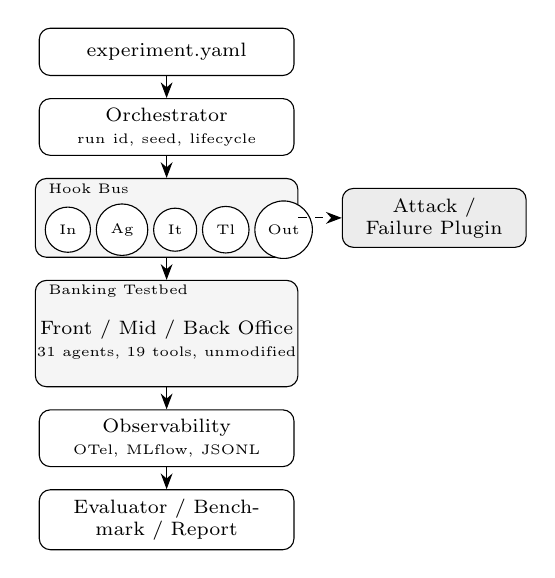
\begin{tikzpicture}[
    box/.style={draw, rounded corners, minimum height=0.6cm, text width=3.0cm, align=center, font=\scriptsize, fill=white},
    node distance=0.28cm,
    >={Stealth[length=2mm]}
]
\node[box] (cfg) {experiment.yaml};
\node[box, below=of cfg] (orch) {Orchestrator\\ \tiny run id, seed, lifecycle};
\node[draw, rounded corners, below=of orch, minimum height=1.0cm, text width=3.1cm, align=center, fill=gray!8] (hb) {};
\node[font=\tiny, above=0.05cm of hb.north west, anchor=north west, xshift=0.05cm] {Hook Bus};
\node[draw, circle, fill=white, font=\tiny, minimum size=0.42cm] (in) at ($(hb.west)+(0.42cm,-0.15cm)$) {In};
\node[draw, circle, fill=white, font=\tiny, minimum size=0.42cm, right=0.06cm of in] (ag) {Ag};
\node[draw, circle, fill=white, font=\tiny, minimum size=0.42cm, right=0.06cm of ag] (it) {It};
\node[draw, circle, fill=white, font=\tiny, minimum size=0.42cm, right=0.06cm of it] (tl) {Tl};
\node[draw, circle, fill=white, font=\tiny, minimum size=0.42cm, right=0.06cm of tl] (out) {Out};
\node[box, right=0.55cm of hb, fill=gray!15, text width=2.1cm] (atk) {Attack / Failure Plugin};
\node[draw, rounded corners, below=of hb, minimum height=1.35cm, text width=3.1cm, align=center, fill=gray!8] (bank) {};
\node[font=\tiny, above=0.06cm of bank.north west, anchor=north west, xshift=0.05cm] {Banking Testbed};
\node[font=\scriptsize, align=center] at ($(bank.center)+(0,-0.08cm)$) {Front / Mid / Back Office\\ \tiny 31 agents, 19 tools, unmodified};
\node[box, below=of bank] (obs) {Observability\\ \tiny OTel, MLflow, JSONL};
\node[box, below=of obs] (eval) {Evaluator / Benchmark / Report};
\draw[->] (cfg) -- (orch);
\draw[->] (orch) -- (hb.north);
\draw[->, dashed] (hb.east) -- (atk.west);
\draw[->] (hb.south) -- (bank.north);
\draw[->] (bank.south) -- (obs.north);
\draw[->] (obs.south) -- (eval.north);
\end{tikzpicture}
\caption{MANTIS pipeline. Every run passes through the same five-point hook bus regardless of banking domain; an attack or failure plugin attaches to the bus and is dispatched alongside the standard observability plugin, without touching the banking agents beneath it.}
\label{fig:architecture}
\end{figure}

\subsection{Banking Runtime Adapter and Domain Coverage}
The banking runtime adapter presents a single interface -- \texttt{inventory()}, \texttt{workflows()}, and \texttt{build()} -- over three domains. The front office covers real-time transaction monitoring, fraud detection, compliance, and a customer-service chatbot, comprising 11 agents. The mid office covers operations planning and representative-assist workflows, comprising 12 agents. The back office covers end-of-day reconciliation and settlement, comprising 8 agents. Across the three domains, agents call 19 distinct banking tools, from read operations such as retrieving a customer's transaction history to write operations with a direct financial side effect, such as executing a transfer or posting a ledger update. The inventory returned by the adapter is introspected live from the tool modules and the agent registry at call time, rather than maintained as a hand-authored list, so that the reported system surface cannot silently drift from the deployed system.

\subsection{Hook Bus and Five Control Points}
The hook bus dispatches a typed context object -- carrying a run identifier, trace identifier, workflow identifier, the control-point stage, a source and target, a payload, and free-form metadata -- to every registered plugin whose declared stages match the current control point. A plugin returns one of five actions: continue, mutate, skip, deny, or error. When a plugin mutates the payload, the mutated version is passed to the next plugin in the chain, and the fact that a mutation (or skip, deny, or error) occurred is recorded in the context metadata so that a plugin registered later in the same dispatch -- notably the observability plugin -- can distinguish a genuinely adversarial event from an ordinary one, rather than simply observing an already-mutated payload indistinguishable from a normal one. The five control points -- input, agent, interaction, tool, and output -- are chosen to bracket every externally observable transition in the agent lifecycle: raw input before any agent reasons about it, an agent's invocation of the underlying model, the message an agent sends to or receives from that model, a tool call and its result, and the final output returned to the caller. A coverage report records, per run, how many times each of the ten before/after hook points fired and which plugins acted on each, which is itself a queryable artifact for confirming that a given experiment configuration actually exercised the control point it claimed to.

\subsection{Attack and Failure Plugins}
Four attack plugins are implemented against the same interface. \textbf{Prompt injection} intercepts raw input at the input control point and injects adversarial instructions before the front-office transaction monitor reasons about a transaction. \textbf{Message spoofing} intercepts the interaction control point -- an agent's outgoing call to the underlying model -- and substitutes a fabricated message, for example a false compliance-clearance signal, into a specific agent's context. \textbf{Route confusion} intercepts a routing tool call and forces execution to a different downstream agent than the one the orchestration logic selected, for example bypassing a compliance step entirely. \textbf{Tool-parameter mutation} intercepts a tool call directly and rewrites its arguments, for example redirecting the destination account on a funds transfer, before the call reaches the banking backend. This fourth plugin is shipped as two configurations rather than one: the front-office configuration above, and a back-office configuration that instead mutates the destination batch identifier of an end-of-day ledger-posting call, redirecting a validated batch's ledger write onto a second, unvalidated batch already present in the domain data -- a confused-deputy attack on settlement rather than on payments, and, together with prompt injection's and message spoofing's front- and mid-office targets, giving five shipped attack configurations that span all three banking domains. A sixth plugin family implements ordinary reliability failures -- delay, timeout, and malformed results -- so that an evaluator can separate a security-caused anomaly from a routine fault. Every attack plugin declares the control points and parameters it supports; the three plugins above whose target is a specific tool call additionally specify that tool through the evaluation schema's expected-tools field, so that \texttt{mantis -{}-evaluate} can report automatically whether the workflow ever reached the point the attack targets, rather than requiring manual inspection of the transcript to notice that it did not -- a distinction Section~\ref{sec:results} shows is not merely hypothetical.

\subsection{Observability Pipeline}
Every hook dispatch is mapped to one of seven typed event families: experiment (run-level start/end, configuration hash, seed, and status), workflow (start, end, and routing decisions, tagged with business domain and terminal outcome), agent (start, end, and error, with latency), interaction (message sent to, received from, or mutated en route to the underlying model), tool (call, result, and error, tagged with operation type, risk level, data sensitivity, and financial side effect), security (an \texttt{ATTACK\_INJECTED} event whenever a plugin took a non-trivial action, carrying the stage, target, plugin, and observed effect), and evaluation (the score each automated evaluator assigned, with a reference to its evidence). Every event is written as a line of portable JSON so that trace analysis never depends on a specific backend, in addition to being exported as OpenTelemetry spans and as an MLflow run carrying the same configuration hash and seed for cross-referencing.

\subsection{Evaluation and Benchmarking Framework}
An automated evaluator reads a run's trace and reports three scores: trace completeness (whether the mandatory workflow, agent, and tool events are present), tool-use correctness (whether every tool the configuration marked as expected was actually called, and no tool marked as forbidden was called), and workflow outcome (whether the terminal state the run actually reached -- inferred from the last business-significant tool invoked, such as a manual-review submission or a transfer execution -- matches the configuration's expected terminal state). A benchmark runner executes a configuration a specified number of times at a specified concurrency and reports latency and throughput; a campaign command sweeps every configuration in a directory, isolates each run's artifacts, and produces one consolidated, human-readable report scoring every experiment side by side.

\subsection{Reproducibility}
Every run manifest records a SHA-256 hash of the fully normalized configuration, the configured random seed, and, as of this work, the Python interpreter version, the installed version of every framework-critical dependency, and the source repository's current commit, so that a reported result can always be traced back to the exact code and environment that produced it. Because the underlying agents are backed by a live LLM, an identical seed narrows but does not eliminate run-to-run variance in exact wording; evaluators are accordingly designed to score bounded, semantic properties -- which tools were called, what terminal state was reached -- rather than exact text matches.

\section{Experimental Results}
\label{sec:results}

\subsection{Implementation Status}
All components described in Section III are implemented and have been exercised end to end against a live backend, in addition to an offline automated test suite of 112 unit, contract, and regression tests plus 13 tests for the standalone banking backend, all of which run in seconds without a live model or backend. A continuous-integration workflow runs this offline suite plus a live execution of one attacked scenario against the real multi-agent pipeline on every push, using the mock model described in \S~\ref{sec:mock-model} so that the check needs no API credential; a failure of that check means an attack plugin stopped actually firing, not merely that a process exited non-zero. This section reports live-verified evidence gathered against both a live backend and, where noted, live model calls; Section~\ref{sec:full-campaign} describes what remains before this evidence is a statistically established evaluation campaign rather than a set of targeted observations.

\subsection{Preliminary, Live-Verified Evidence}
Hook coverage was measured across representative front-, mid-, and back-office runs; all ten before/after hook points recorded at least one hit in every run, confirming that no control point is silently unreachable for the workflows exercised. A campaign run of all three domain baselines together with all six shipped attack configurations -- exercised through the campaign command described in \S~III-F, which we found and fixed a run-name-resolution bug in while doing so, since it had silently aggregated zero of three baseline runs into their campaign report by assuming a config's file name always matches the \texttt{experiment.name} it declares -- completed with every run reaching a terminal workflow state and, for every attack, an \texttt{ATTACK\_INJECTED} security event confirming the plugin executed, across all three banking domains rather than the two the plugin set originally covered.

That last check -- grepping the trace for the security event an attack actually emits, rather than trusting that its process exited zero -- is not a formality. Applying it to the route-confusion plugin specifically surfaced a real, previously-undetected bug: the plugin matched a rerouted transfer against payload keys \texttt{target\_agent} or \texttt{agent\_id}, but the underlying framework's own transfer tool (\texttt{google.adk.tools.transfer\_to\_agent\_tool}) takes a single argument named \texttt{agent\_name}. Every historical run of this plugin, including ones executed against a live model with the LLM genuinely invoking a real transfer, therefore reached the intended tool call without the plugin ever once matching it -- a silent no-op that a process-exit-code check cannot distinguish from success, and that the previous version of this paper reported (incorrectly, on the strength of exactly that weaker check) as a verified attack effect. We diagnosed this directly against the installed framework's source, including its agent-relatedness resolution logic that restricts a transfer to parent, child, or sibling agents, corrected the plugin to match \texttt{agent\_name}, and added a regression test against the corrected key together with an \texttt{expected\_tools} ground-truth entry (\S~III-D) so that a future occurrence of this failure mode -- the target tool never being reached, for whatever reason -- is flagged by \texttt{mantis -{}-evaluate} automatically rather than depending on a human to grep the trace. A live-model re-verification that the corrected plugin now intercepts and reroutes a genuine transfer is pending API access at the time of writing.

The message-spoofing plugin, by contrast, was independently verified against a live model to emit an \texttt{ATTACK\_INJECTED} event together with a \texttt{MESSAGE\_MUTATE} interaction event correctly attributing the mutation to the targeted agent, and that evidence stands. The tool-parameter-mutation plugin's own historical live run surfaced a different, non-bug nuance in the same spirit: in that run the model reasoned about the suspicious transaction pattern but never called \texttt{execute\_transfer} at all, so the mutation plugin had no tool call to intercept -- legitimate model behavior, not a defect, but exactly the kind of single-run non-determinism that motivates both the \texttt{expected\_tools} ground truth added for this plugin and the repeated-trial measurements in \S~\ref{sec:full-campaign}.

\subsection{Isolating Overhead from LLM Latency}
\label{sec:mock-model}
To address the confound above, we implemented a mock model that an experimenter opts into per benchmark configuration (\texttt{MANTIS\_MOCK\_LLM=1} or a config-level flag), removing live model sampling entirely. The mock is tool-calling-capable, not text-only: on an agent's first turn it emits a function call against one of that agent's declared tools with a plausible dummy argument set drawn from the real banking tool schemas, so the tool control point -- and any tool-stage attack plugin -- is exercised the same way a real model call would exercise it, then returns a final text response once a tool result is present. It is deliberately not a planner: it has no access to which agent is calling it, and the underlying framework only allows its \texttt{transfer\_to\_agent} routing tool between agents that are parent, child, or sibling of one another, so a mock-driven run reliably reaches the tool control point on whichever agent runs first but does not reliably route itself deep into a multi-agent hierarchy the way a reasoning model does. This is why the campaign evidence in \S~IV-B reports that every attack's target tool was reachable in principle (via \texttt{expected\_tools}) rather than claiming the mock run demonstrated every attack's live effect; only prompt injection's unconditional input-stage path is checkable under mock model, and it is what our continuous-integration workflow (\S~IV-A) checks on every push for exactly that reason.

An initial off/full comparison with live model sampling removed was, itself, informative in a different way: at four repetitions and concurrency 2, the comparison remained noisy and backwards from what an overhead claim would predict (off: 8.53\,s average; full: 6.68\,s average). Investigating why surfaced a genuine confound in our own benchmark methodology rather than in the system under test: running multiple full Python-interpreter-plus-framework subprocesses concurrently on a single machine introduces shared-CPU contention that inflates every concurrent run's latency by an amount unrelated to instrumentation, and that we verified directly -- the same configuration at concurrency 4 measured 7--10\,s per run, against 6.5--6.7\,s at concurrency 1 for the identical work. Repeating the comparison at concurrency 1 (serial execution, no contention) and 20 repetitions per side gives a clean result in the expected direction: off averaged 6.517\,s ($\sigma=0.163$\,s; P50 6.507\,s, P90 6.708\,s, P99 6.865\,s) against full's 6.695\,s ($\sigma=0.229$\,s; P50 6.669\,s, P90 7.016\,s, P99 7.320\,s) across 20/20 successful runs each -- a difference of 0.178\,s, or roughly 2.7\% of the off baseline.

That end-to-end figure still bundles trace serialization, file I/O, and OpenTelemetry span creation together with the hook bus's own dispatch cost, so we separately instrumented the hook bus to record, per run, the cumulative wall-clock time spent inside the observability plugin's own \texttt{apply()} calls -- a direct measurement of instrumentation cost that needs no off/full diff and is consequently immune to the process-startup and contention confounds above, since it never depends on comparing two separate processes at all. Across ten repeated trials of a representative front-office run, this direct measurement gave a median instrumentation overhead of 0.195\% of total run duration (mean 0.379\%, $\sigma=0.515\%$; nine of ten trials fell between 0.17\% and 0.43\%, with one outlier at 1.83\% consistent with ordinary OS scheduling jitter on a shared development machine). That the direct figure ($\approx$0.2--0.4\%) is smaller than the end-to-end diff ($\approx$2.7\%) is itself informative: the gap is attributable to trace-write I/O and span export, which the end-to-end comparison necessarily includes and the direct hook-dispatch measurement necessarily excludes, rather than to any inconsistency between the two methods -- both figures place instrumentation overhead well under 5\% of end-to-end run time, and neither depends on live model sampling.

\subsection{Volume Scaling}
We also implemented a scaling mode in which the benchmark runner executes a configurable list of repetition counts at a fixed concurrency, rather than a single repetition count, so throughput and latency can be reported as a function of transaction volume instead of a single point estimate. Run with the mock model at concurrency 2 across 1, 2, 4, and 8 repetitions, throughput rose sharply from 1 to 2 repetitions (0.154 to 0.288 runs/s) as fixed per-batch startup cost was amortized over more transactions, then plateaued and drifted slightly downward through 4 and 8 repetitions (0.287 and 0.277 runs/s respectively) as average per-run latency correspondingly crept up (6.48\,s, 6.95\,s, 6.98\,s, 7.22\,s) -- a sensible curve shape (an early amortization gain that does not continue indefinitely at a fixed concurrency level on a fixed machine), though generated with the mock model and at a small number of volume levels, not yet with a live model or across all three banking domains.

\subsection{Remaining Work Toward a Full Evaluation Campaign}
\label{sec:full-campaign}
Since the preliminary pass of this evaluation, direct hook-dispatch instrumentation timing has replaced the process-bootstrap-confounded off/full comparison as the primary overhead measurement (\S~\ref{sec:mock-model}), the mock model has become tool-calling-capable, and the attack-plugin and campaign-tooling bugs described in \S~IV-B have been fixed and covered by regression tests. Two things remain before the evidence in this section is a statistically established evaluation campaign rather than a set of targeted, repeated-but-still-few-trial observations.

First, and most concretely: a live-model re-verification that the corrected route-confusion plugin now intercepts and reroutes a genuine transfer end to end, together with a fresh live-model run of every other attack configuration against the current codebase, is pending API credential access in the environment this paper was written in. The plugin logic itself is verified correct against the framework's actual argument schema (\S~IV-B) and by a targeted regression test, but that is not a substitute for observing the corrected behavior against a live reasoning model, and we report it as outstanding rather than assumed.

Second, repeated-trial statistics with a mean and a variance are now genuinely reported for benchmark latency and throughput (\S~IV-C, IV-D) and, separately, for direct instrumentation overhead (ten trials, \S~\ref{sec:mock-model}) -- but not yet for attack \emph{efficacy} itself (did the attack produce its intended downstream effect, not merely did it fire) repeated across many trials per domain and attack family with a live model. The mock model that makes repeated, zero-cost trials practical is deterministic by design, so repeating a mock-driven security outcome many times would show zero variance and would not be informative about the live-model variance this measurement is meant to characterize; that specific combination -- many repeated trials, per domain and attack family, against a live model, scoring effect rather than firing alone -- is the concrete piece of statistical rigor that remains, and it is a live-model-access question rather than an implementation gap. We report the current state of each measurement rather than a projected final result, because presenting a small number of trials as though they were a statistically established finding would overstate what has actually been shown.

\section{Conclusion}
We presented MANTIS, a configuration-driven testbed that instruments a realistic, unmodified banking multi-agent system at five fixed control points, so that adversarial and failure experiments are declared in YAML rather than implemented as changes to business logic. The testbed's banking runtime adapter, hook bus, five attack configurations across three domains, observability pipeline, and evaluation and benchmarking framework are implemented and verified end to end, including a reproducibility mechanism that records the environment, not only the configuration, behind every run. Live-verified evidence confirms that every control point is reachable; it also surfaced, and let us fix, a real bug in one attack plugin that had silently never fired in any prior run because it matched the wrong argument name against the underlying agent framework's actual transfer tool -- a finding that is itself evidence for why verifying an attack's emitted security event, rather than trusting a clean process exit, has to be load-bearing in a testbed like this one, not optional rigor. A tool-calling mock model and a volume-scaling benchmark mode isolate instrumentation overhead from LLM sampling latency and per-process startup cost respectively, arriving at a direct, repeated-trial measurement of instrumentation overhead at a median of 0.195\% of run duration, corroborated by a contention-controlled end-to-end comparison at roughly 2.7\% in the same direction. What remains toward a full statistical evaluation campaign is now narrower and more concrete than when this overhead question was still open: a live-model re-verification of the corrected plugin and of the other attack configurations against current code, and repeated-trial, mean-and-variance statistics for attack \emph{efficacy} specifically -- as opposed to the latency and instrumentation-overhead statistics already reported -- across domains and attack families with a live model, since a deterministic mock cannot itself characterize live-model variance. Future work extends this testbed along the directions its interfaces were explicitly designed to support without modification: a minimal schema-driven UI over the existing CLI, additional observability exporters, security-mechanism (guardrail and policy) plugins evaluated through the same plugin interface as the attacks in this paper, and a Zero Trust Backplane that consumes the same application inventory and control-point metadata described in Section III to generate and enforce access policy as a separate research contribution.

\section*{Acknowledgment}
% Insert acknowledgment of funding sources and individual contributions here.

\begin{thebibliography}{00}

\bibitem{anomaly_detection_finance}
X.~Zhang et al., ``Enhancing Anomaly Detection in Financial Markets with an LLM-based Multi-Agent Framework,'' \emph{arXiv preprint arXiv:2403.19735}, 2024.

\bibitem{masca_credit}
``MASCA: LLM based-Multi Agents System for Credit Assessment,'' \emph{arXiv preprint arXiv:2507.22758}, 2025.

\bibitem{prompt_infection}
D.~Lee and M.~Tiwari, ``Prompt Infection: LLM-to-LLM Prompt Injection within Multi-Agent Systems,'' \emph{arXiv preprint arXiv:2410.07283}, 2024.

\bibitem{aitm_communication_attacks}
``Red-Teaming LLM Multi-Agent Systems via Communication Attacks,'' in \emph{Findings of the Association for Computational Linguistics: ACL 2025}, arXiv preprint arXiv:2502.14847.

\bibitem{agentic_security_survey}
``A Survey on Agentic Security: Applications, Threats and Defenses,'' \emph{arXiv preprint arXiv:2510.06445}, 2025.

\bibitem{security_considerations_mas}
``Security Considerations for Multi-agent Systems,'' \emph{arXiv preprint arXiv:2603.09002}, 2026.

\bibitem{redagentbench}
``REDAgentBench: Executable Red Teaming and Faithful Measurement of LLM Agent Systems,'' \emph{arXiv preprint arXiv:2608.10669}, 2026.

\bibitem{nist_zero_trust}
S.~Rose, O.~Borchert, S.~Mitchell, and S.~Connelly, ``Zero Trust Architecture,'' NIST Special Publication 800-207, National Institute of Standards and Technology, Aug. 2020.

\bibitem{zero_trust_agentic_identity}
``A Novel Zero-Trust Identity Framework for Agentic AI: Decentralized Authentication and Fine-Grained Access Control,'' \emph{arXiv preprint arXiv:2505.19301}, 2025.

\end{thebibliography}
\vspace{12pt}


\end{document}
